\documentclass[11pt]{article}
\usepackage{mypackages}
\begin{document}

\maketitle

\section{Deep Learning}\label{sec:deep_learning}

In section \ref{sec:et} we mentioned that
a \textit{neural network} can be used as a function approximator.
This means the neural network can be seen as a function $f^\sim(x)$ that approximates a
function $f(x)$ and we will be using neural networks to estimate
both the state-value function and the policy.
We will present Deep Learning in this section with regards to the book \cite{DeepLearningBook} and the slides, \cite{IgelConv}, by Christian Igel
from the University of Copenhagen.

\subsection{Layers, Neurons and Connections}\label{sec:lnc}

To approximate $f(x)$ the network uses a combination of simpler functions.
More formally, a neural network consists of a number of \textit{layers},
that each represent a function $f^i : \R^{d} \to \R^k$.
This means the network can be seen as a composition of the functions
\begin{equation}\label{eq:layers}
    f^\sim(x) = f^n(f^{n-1}( \cdots f^1(x) \cdots))
\end{equation}
for a network with $n$ layers.
The layers of the network inbetween the input and output layer, are called
\textit{hidden layers}, because we won't be directly seeing their output.

In equation \ref{eq:layers}, each of the layers describe a simple function
and by combining the results of the simpler functions, the neural network
is able to solve complex problems.
This structure is a \textit{hierarchy of concepts}, where each concept can be described in terms
of simpler concepts, provided by the previous layers.
Each layer consists of a number of \textit{neurons} that are connected to the
neurons of the next layer.
\begin{figure}[!h]
    \centering
    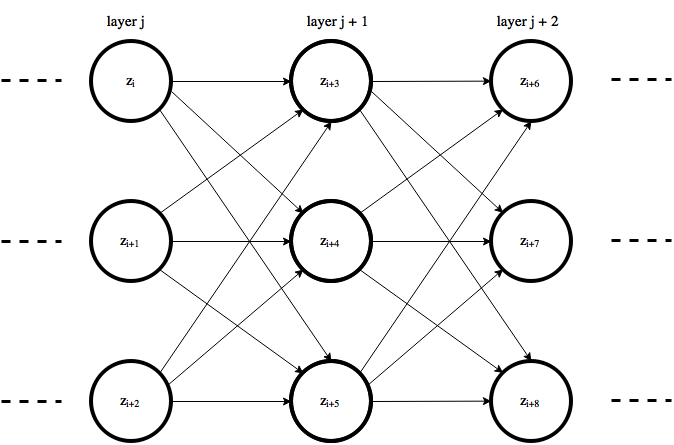
\includegraphics[width=12cm]{include/layers.png}
    \caption{A series of layers in a fully connected neural network, where each layer consists of three neurons.}
    \label{fig:layers}
\end{figure}

A neuron is a unit that transforms a series of input signals into a single output signal.
Each of the input signals are sent through a \textit{weighted connection}, which means
that the input $a_i$ to a neuron $z_i$ is given by
\begin{equation}
    a_i = \sum\limits_{j} w_{ij}* z_j
\end{equation}
for all neurons $z_j$ in the previous layer with a connection to $z_i$.

The purpose of each of the hidden layers is to extract some features from the input.
To achieve this an \textit{activation function}, $h: \R^d \to \R$, is used on the weighted
input, that can either highlight or dampen
certain properties of the input.
Combining the features extracted by the hidden layers is what enables the network
to approximate $f(x)$.
The only way to change the network is by altering the weighted connections
between the neurons, and the general idea is to change the weights such that
$f^\sim(x)$ varies the least from $f(x)$ for all $x$.
To update the weights of the networks we will be using gradient ascent
for the Actor-Critic method and RMSpropagation for the A3C algorithm,
as presented in section \ref{sec:actor_critic_el} and \ref{sec:a3c}.
%%%% A drawing of a neuron “up close”
\begin{figure}[!h]
    \centering
    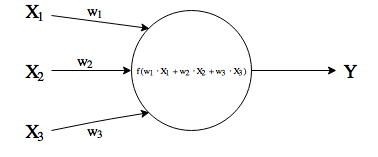
\includegraphics[width=12cm]{include/neuron.png}
    \caption{The structure of a single neuron with activation function $h$.}
    \label{fig:neuron}
\end{figure}

The choice of activation function depends on the task the
network is supposed to solve.
In our case we wish to learn a policy and estimate the value of a state.
The policy is a probability distribution, and we will be using a softmax function
to emulate this, as described in section \ref{sec:improv}, in the final layer.
The softmax function is defined as
\begin{equation}
    \text{softmax}(x) = \frac{e^{h(a_i)}}{\sum\limits_{\ell} e^{h(a_\ell)}}
\end{equation}
for each of the $\ell$ actions we wish to assign a probability.
Here the weighted connection from the previous layer, works as
a numerical preference for each of the actions.
The softmax function is a generalization of the sigmoid function, $\frac{1}{1 + e^{-x}}$,
which is shown below.
\begin{figure}[!h]
    \centering
    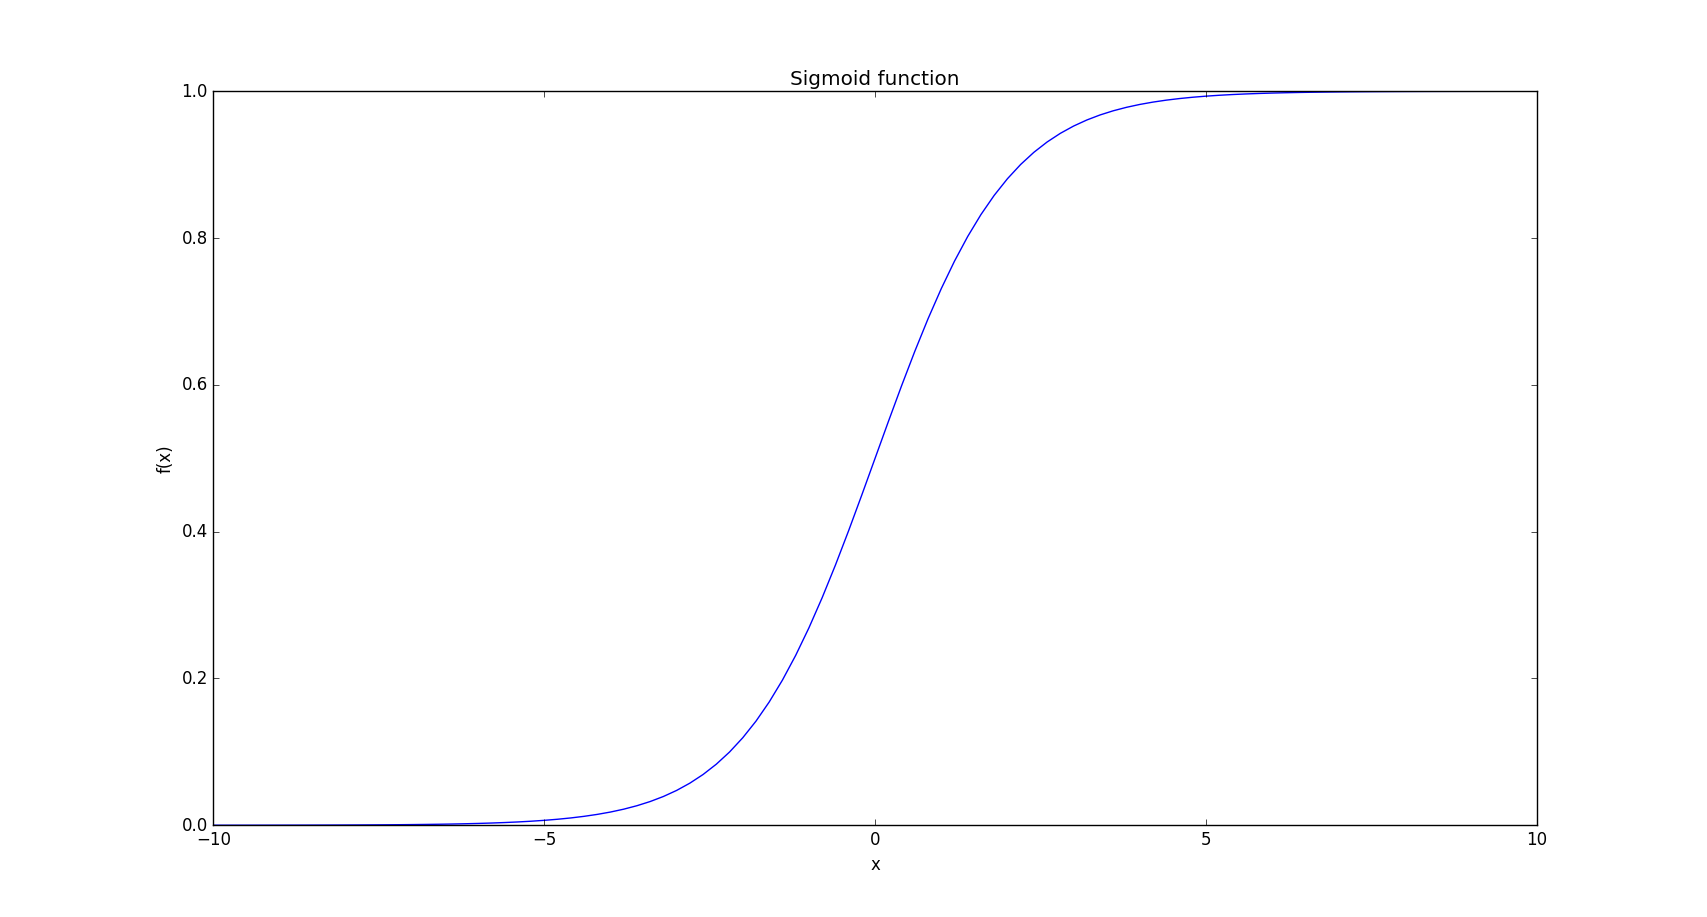
\includegraphics[width=15cm]{include/sigmoid.png}
    \caption{Plot of the sigmoid function.}
    \label{fig:softmax}
\end{figure}

The value estimate should only be a single output, and therefore we have chosen to
let the output of the neural network that approximates $v_\pi(s)$ be given
as the sum of the output of the neurons in the second to last layer.

In the hidden layers we will be using the \textit{Rectified
Linear Unit} (ReLU) as an activator.
The ReLU is defined as
\begin{equation}
    f(x) = \max(0,x)
\end{equation}
A benefit of the ReLU is that the gradient is always constant - 
if $x \leq 0$ then the gradient is 0, and if $x > 0$ the gradient is 1.
This can result in faster learning, since the gradient won't change even
though the weights of the network changes.
\begin{figure}[!h]
    \centering
    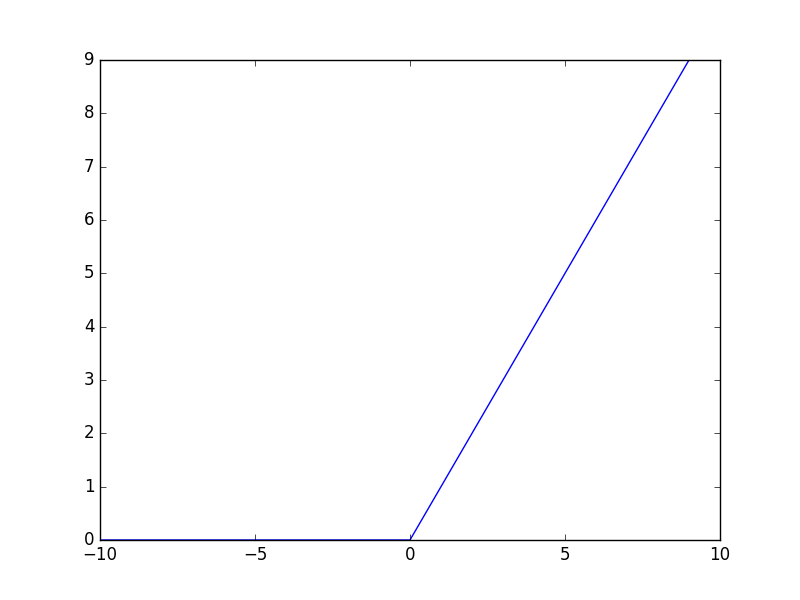
\includegraphics[width=15cm]{include/relu.png}
    \caption{Plot of the ReLU function.}
    \label{fig:relu}
\end{figure}

The choice of activation function defines the role of each layer,
with the overall goal being to perform ongoing transformations
to the input, until the network is able to use the extracted
features to make a prediction of the output.

\subsection{Learning from Multidimensional Input}

To process the high dimensional frames from the Atari games we will be using
a \textit{Convolutional} Neural Network (CNN).
In addition to the activation performed in a neural network, a CNN
also performs a \textit{convolution} and a \textit{pooling} of the input in each convolutional layer.

In this project, the input to the CNN will be a two dimensional input with a single
channel - a grayscaled and resized Atari frame.
A convolution in two dimensions of a discrete image $I$ with filter kernel $K$
is given by 
\begin{equation}
    S(i, j) = (I \ast K)(i, j) = \sum\limits_m \sum\limits_n I(m, n) * K(i - m, j - n)
\end{equation}
where the kernel filter $K$ is a function $K : \R^{(d, k)} \to \R$.
A 2D convolutional layer takes advantage of the spatial structure in the input data to contruct a feature map
using the filter.
In a classic Neural Network each neuron has its own weighted connection to each neuron in the subsequent layer,
but in a convolutional layer the neurons share a kernel of weights - the filter $K$ -  which can be represented as
a $d \times k$ dimensional matrix.
$$
K =
\begin{bmatrix}
    w_{1,1 } & w_{1, 2} & \hdots & w_{1, k} \\
    w_{2,1 } & w_{2, 2} & \hdots & w_{2, k} \\
    \vdots   &          & \ddots &          \\
    w_{d,1 } & w_{d, 2} & \hdots & w_{d, k} \\
\end{bmatrix}
$$
Each element in the resulting feature map describes the weighted sum of its neighbouring
pixels.
Due to the spatial structure found in images, performing a neighbourhood operation
can be seen as extracting features from the original input - e.g. finding the
edges in an image by performing a finite center differencing.

For a $4 \times 4$ input image and a $3 \times 3$ kernel filter the convolution
would be given by
%%% 2d convolution
\begin{figure}[!h]
    \centering
    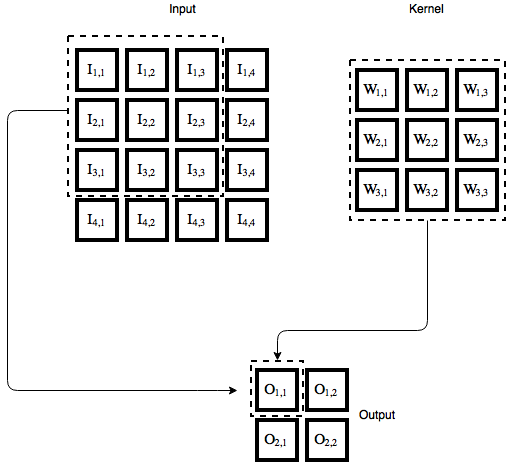
\includegraphics[width=10cm]{include/conv_2.png}
    \caption{A 2D convolution on an image which produces a feature map.}
    \label{fig:conv}
\end{figure}
\newpage
A problem with the convolution shown in figure \ref{fig:conv} is that
pixels at the boundary of the image are lost.
To deal with this issue we make use of zero padding.
By adding zeros to the border of each image, until the kernel
filter fits around each pixel, the image can maintain its dimensions, since
only the padding will be list in the convolution.
%%% Zero padded 2d convolution
\begin{figure}[H]
    \centering
    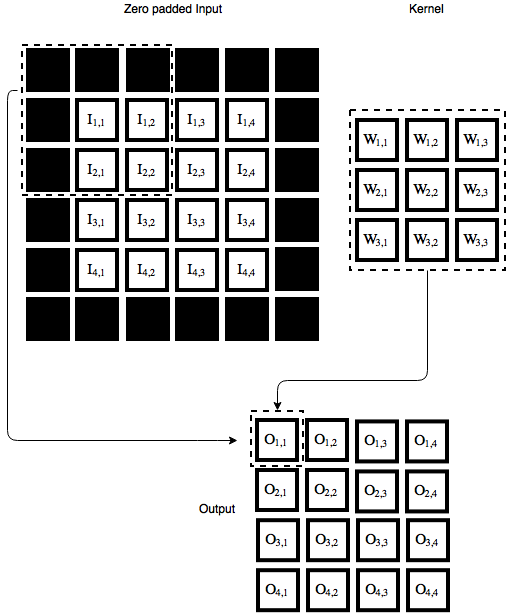
\includegraphics[width=10cm]{include/conv_2_zero_pad.png}
    \caption{The effect of using zero padding on the input image,
             before performing the convolution.}
    \label{fig:conv2}
\end{figure}
Each element in the resulting feature map contains information about
its neighbouring pixels, which means we can reduce the dimensionality
without losing as much information as if we reduced it before performing the convolution.
The reduction performed is called a \textit{pooling} and attempts to retain
as much information as possible, from the feature map produced by the previous convolution. 
A common pooling scheme is to let every resulting element be the maximum
or average value of an area of the input.
\begin{figure}[H]
    \centering
    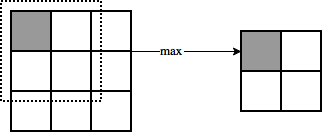
\includegraphics[width=10cm]{include/pooling.png}
    \caption{A max-pooling performed on an image.}
\end{figure}
The pooling is performed to support \textit{translation invariance},
which is used to make sure the features of the input are able to
be extracted, regardless of their position in the feature map.
In an Atari game most objects move, while maintaining their original shape.
Thus, being able to
extract information about objects independent of their position is very useful.

Instead of performing both a pooling and a convolutions in two separate steps,
we will be using convolutions \textit{with stride}.
The stride determines the movement of the kernel filter, which means that
using a stride of $n$, results in the kernel filter skipping $n$ elements 
while computing the convolution.
%%%%% Strides
\begin{figure}[!h]\label{con2}
    \centering
    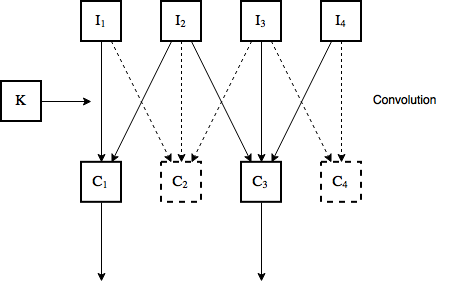
\includegraphics[width=10cm]{include/strides.png}
    \caption{A convolution in one dimension, using a stride of 2.
             This is effectively halving the size of the input, since
             the convolution is skipping every second element.}
    \label{fig:conv}
\end{figure}
Here the convolution skips every second element, resulting in a downsampling
of the input.
In two dimensions a convolution can be seen as the kernel moving across
an image, which means the stride is the amount of pixels the filter is moved.
Therefore the dimensions of an image can be halved by using a stride of $(2, 2)$, meaning
the stride is performed in both dimensions.

The pooling operation usually computes the maximum or average of a region of
a feature map, and using convolution with strides emulates
this behaviour since the convolution
is seen as a weighted sum of neighbouring pixels.


%%% Move this to after Policy Gradients
%\subsubsection{Updating the weights of the network}

%A neural network is trained to minimize its total loss based on its \textit{loss
%function}.
%A loss function $\mathcal{L} : \R^K \to \R$ is supposed to describe how close the
%predictions are to the true result.
%In the reinforcement learning setting it is often difficult to estimate the
%true result.
%E.g. for a policy aproximator $\pi^{\sim}(A_t | S_t)$ we want to use the knowledge
%of wether or not action $A_t$ was  chosen in state $S_t$ to determine
%whether the probability of taking $A_t$ should be increased or decreased to
%reduce the loss of the network.
%Therefore the weights of the connections in the network are typically updated
%in a direction in the weight space.
%This direction describes how the weights should be updated to increases the
%probability of repeating the action $A_t$ the most on future visits to
%state $S_t$\cite{RLbook}.
%To find the direction we would use the \textit{gradient} of the probability of
%taking the action actually taken, since it exactly describes how to increate
%this probability.
%
%Now, this would increase the chance of picking action $A_t$ in state $S_t$ again,
%but we really only want to pick actions again that lead to a good return.
%Therefore the probability is generally updated proportionally to the
%return, since the network will then learn to favor actions that provide
%the highest return.
%

\documentclass[11pt]{article}
\usepackage{mypackages}
\begin{document}


\subsection{Updating the weights of a network}

In section \ref{sec:actor_critic} and \ref{sec:a3c} we discussed different
approaches available to update the weights of the policy and value estimator.
These approaches are based on the directional values
expressed by the gradient of the estimator, or an error measure containing
the estimator.
Taking the gradient of a function $f : \R^n \to \R$ with respect to
some parameters $x \in \R^n$ is given by
\begin{equation}
    \nabla_x f(x)
    = \begin{pmatrix}
        \frac{\partial f(x)}{\partial x_1}\\
        \frac{\partial f(x)}{\partial x_2}\\
        \vdots\\
        \frac{\partial f(x)}{\partial x_n}
      \end{pmatrix}
\end{equation}

Now, in a neural network it is difficult to take the gradient of the
entire network at once, since it consists of a number of layers
using different activation functions and a lot of parameters.
To solve this issue the general approach to computing the gradient of a network
is to use \textit{back-propagation} as presented in \cite{IgelBackProp}
and \cite{DeepLearningBook}.

Consider a network consisting of $d$ input neurons, $M$ hidden neurons and $K$ output neurons,
estimating the function $f : \R^d \to \R^K$.
Each neuron can be denoted as $z_i$, where neurons for which $i \leq d$ are the input neurons, $d < i \leq M + d$ are the hiden neurons
and $M + d < i \leq M + d + K$ are the output neurons.
As described in section \ref{sec:lnc} each neuron $z_i$ can be seen as a weighted activation of its input.
For the neurons in the hidden layers and the output layer, this means $z_i = h(a_i)$, where 
$a_i = \sum_{j} w_{ij} * z_{j}$ is the weighted sum of the input to the i'th neuron and $h$ is an arbitrary
activation function.

Previously we updated the weights of an estimator with regards to some performance measure $\rho$ 
describing how well the policy and value functions are performing. 
Now, we want to find the directional changes for all weights in the network
in regards to the performance measure.
If all $h$ in the network are differentiable this results in the partial derivatives
\begin{equation}\label{part}
    \frac{\partial \rho}{\partial w_{ij}}
\end{equation}
describing the directional change for each weighted connection in the network from $z_j$ to $z_i$.

If we start by looking at this partial derivative in the $K$ output neurons of the
neural network, we can apply the chain rule of calculus to equation \ref{part},
\begin{equation}
    \frac{\partial \rho}{\partial w_{ij}} = \frac{\partial \rho}{\partial a_i} \frac{\partial a_i}{\partial w_{ij}} 
\end{equation}
since $w_{ij}$ is a part of $a_i$.
$\frac{\partial \rho}{\partial a_i}$ is denoted as $\delta_i$ and have that $\frac{\partial a_i}{\partial w_{ij}} = z_j$ since
$\frac{\partial a_i}{\partial w_{ij}} = \frac{\partial}{\partial w_{ij}} \sum_{d} w_{id} * z_d = z_j$.
This means
\begin{equation}\label{eq:der}
    \frac{\partial \rho}{\partial w_{ij}} = \delta_i * z_j  
\end{equation}
For each of the output units, $\delta_i$ can be found as
\begin{equation}
    \begin{aligned}
        \delta_i & = \frac{\partial \rho}{\partial a_i}\\
        & = \frac{\partial \rho}{\partial z_i} \frac{\partial z_i}{\partial a_i}\\
        & = h'(a_i) \frac{\partial \rho}{\partial z_i} 
    \end{aligned}
\end{equation}
since $\frac{\partial z_i}{\partial a_i} =  \frac{\partial}{\partial a_i} h(a_i) = h'(a_i)$.
Therefore the partial derivative of the performance measure with respect to a weight from
an output neuron can be found as
\begin{equation}
    \frac{\partial \rho}{\partial w_{ij}} = h'(a_i) \frac{\partial \rho}{\partial z_i} * z_j
\end{equation}
This only holds for the output neurons because their output isn't
used by any other neuron.
For the hidden neurons we have to take all subsequent neurons into account as
well, since their output is propagated forward through the network.
Thus,
\begin{equation}
    \delta_i = \sum\limits_{k=i+1}^{M + d + K} \frac{\partial \rho}{\partial a_k} \frac{\partial a_k}{\partial a_i} 
\end{equation}
for all hidden neurons, $z_i$, for which $d > i \leq M + d + K$.
Since $\frac{\partial \rho}{\partial a_k} = \delta_k$ and
$\frac{\partial a_k}{\partial a_i} = \frac{\partial a_k}{\partial z_i} \frac{\partial z_i}{\partial a_i}$ we
can derive $\delta_i$ as
\begin{equation}
    \begin{aligned}
        \delta_i & = \sum\limits_{k=i+1}^{M + d + K} \delta_k \frac{\partial a_k}{\partial z_i} \frac{\partial z_i}{\partial a_i}\\
        & = \sum\limits_{k=i+1}^{M + d + K} \delta_k * w_{ki} *  h'(a_i)\\
        & = h'(a_i) \sum\limits_{k=i+1}^{M + d + K} \delta_k * w_{ki}
    \end{aligned}
\end{equation}
because $\frac{\partial a_k}{\partial z_i} = \frac{\partial}{\partial z_i} \sum_{j} w_{kj} * z_j = w_{ki}$.
Using these equations, we can then compute the partial derivatives for all output and hidden neurons
by computing $\delta$, since we already have access to the value of $z_j$.
However, it is important to note that the partial derivatives have to be computed in the reverse order,
since each derivative in each neuron, $z_j$, is dependant of all derivatives of all later neurons $z_i$ for $j < i$.


%%%% AFSLUTNING %%%%

Now that we have an understanding of the underlying principles of Deep Reinforcement Learning, we can apply it to real problems.
We have presented a lot of theory in the last sections,
with most important aspects being the fundamentals of the Actor-Critic method and how eligibility have a stabilizing effect on learning,
as well as the idea of using asynchronous training to speed up the training process, and lastly
how Deep Learning can be used to estimate a policy and the state-value function

\end{document}

\end{document}
